\documentclass[a4paper,11pt]{article}
\usepackage{amsmath,amsthm,amsfonts,amssymb,amscd,amstext,vmargin,graphics,graphicx,tabularx,multicol} 
\usepackage[francais]{babel}
\usepackage[utf8]{inputenc}  
\usepackage[T1]{fontenc} 
\usepackage{pstricks-add,tikz,tkz-tab,variations}
\usepackage[autolanguage,np]{numprint} 

\setmarginsrb{1.5cm}{0.5cm}{1cm}{0.5cm}{0cm}{0cm}{0cm}{0cm} %Gauche, haut, droite, haut
\newcounter{numexo}
\newcommand{\exo}[1]{\stepcounter{numexo}\noindent{\bf Exercice~\thenumexo} : \marginpar{\hfill /#1}}
\reversemarginpar


\newcounter{enumtabi}
\newcounter{enumtaba}
\newcommand{\q}{\stepcounter{enumtabi} \theenumtabi.  }
\newcommand{\qa}{\stepcounter{enumtaba} (\alph{enumtaba}) }
\newcommand{\initq}{\setcounter{enumtabi}{0}}
\newcommand{\initqa}{\setcounter{enumtaba}{0}}

\newcommand{\be}{\begin{enumerate}}
\newcommand{\ee}{\end{enumerate}}
\newcommand{\bi}{\begin{itemize}}
\newcommand{\ei}{\end{itemize}}
\newcommand{\bp}{\begin{pspicture*}}
\newcommand{\ep}{\end{pspicture*}}
\newcommand{\bt}{\begin{tabular}}
\newcommand{\et}{\end{tabular}}
\renewcommand{\tabularxcolumn}[1]{>{\centering}m{#1}} %(colonne m{} centrée, au lieu de p par défault) 
\newcommand{\tnl}{\tabularnewline}

\newcommand{\bmul}[1]{\begin{multicols}{#1}}
\newcommand{\emul}{\end{multicols}}

\newcommand{\trait}{\noindent \rule{\linewidth}{0.2mm}}
\newcommand{\hs}[1]{\hspace{#1}}
\newcommand{\vs}[1]{\vspace{#1}}

\newcommand{\N}{\mathbb{N}}
\newcommand{\Z}{\mathbb{Z}}
\newcommand{\R}{\mathbb{R}}
\newcommand{\C}{\mathbb{C}}
\newcommand{\Dcal}{\mathcal{D}}
\newcommand{\Ccal}{\mathcal{C}}
\newcommand{\mc}{\mathcal}

\newcommand{\vect}[1]{\overrightarrow{#1}}
\newcommand{\ds}{\displaystyle}
\newcommand{\eq}{\quad \Leftrightarrow \quad}
\newcommand{\vecti}{\vec{\imath}}
\newcommand{\vectj}{\vec{\jmath}}
\newcommand{\Oij}{(O;\vec{\imath}, \vec{\jmath})}
\newcommand{\OIJ}{(O;I,J)}


\newcommand{\reponse}[1][1]{%
\multido{}{#1}{\makebox[\linewidth]{\rule[0pt]{0pt}{20pt}\dotfill}
}}

\newcommand{\titre}[5] 
% #1: titre #2: haut gauche #3: bas gauche #4: haut droite #5: bas droite
{
\noindent #2 \hfill #4 \\
#3 \hfill #5

\vspace{-1.6cm}

\begin{center}\rule{6cm}{0.5mm}\end{center}
\vspace{0.2cm}
\begin{center}{\large{\textbf{#1}}}\end{center}
\begin{center}\rule{6cm}{0.5mm}\end{center}
}



\begin{document}
\pagestyle{empty}

\titre{Contrôle  : Trigonométrie et Théorème de Pythagore}{Nom}{Prénom}{Date}{Classe}
\vspace*{0.5cm}

\exo{1.5} Dans chaque cas, donner la valeur arrondie au degré de $x$.\\
\initqa \qa $sin(x)=0,32$ \hspace*{0.5cm} \qa $tan(x)=36$  \hspace*{0.5cm} \qa $cos(x)=\dfrac{2}{3}$ \\

\vspace*{0.25cm}

\exo{3} Calculer la longueur RT arrondie au millimètre.
\begin{center}
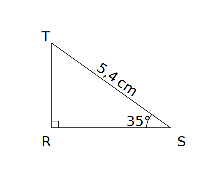
\includegraphics[scale=1.4]{trigo1.eps} 
\end{center}
\vspace*{0.25cm}

\exo{4.5}

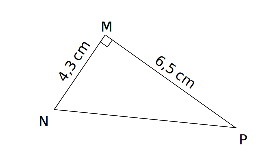
\includegraphics[scale=1.2]{trigo2.eps} \\

\noindent \initqa \qa Calculer la mesure arrondie au degré de l'angle $\widehat{MNP}$.\\
\qa En déduire la mesure arrondie au degré de l'angle $\widehat{MPN}$.\\

\vspace*{0.5cm}

\exo{5} Lors d’une intervention les pompiers doivent atteindre une
fenêtre F située à 18 m du sol en utilisant la grande échelle
[PF].\\
Ils doivent prévoir le réglage de l’échelle.\\
Le pied P de l’échelle est situé sur le camion à 1, 5 m du sol
et à 10 m de l’immeuble.\\

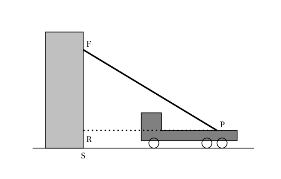
\includegraphics[scale=2.5]{trigo3.eps} \\

\noindent \q Avec les informations ci-dessus, en déduire la longueur RF.\\
\q Déterminer au degré près l’angle que fait l’échelle avec
l’horizontale, c’est à dire l’angle $\widehat{FPR}$.\\
\q L’échelle à une longueur maximale de 25 m. Sera-t-elle assez longue pour atteindre la fenêtre ?\\

\newpage
\vspace*{0.5cm}
\exo{6}

Pour savoir si les feux de croisement de sa voiture sont réglés correctement, Pauline éclaire un mur vertical comme l'illustre le dessin suivant :

\begin{center}
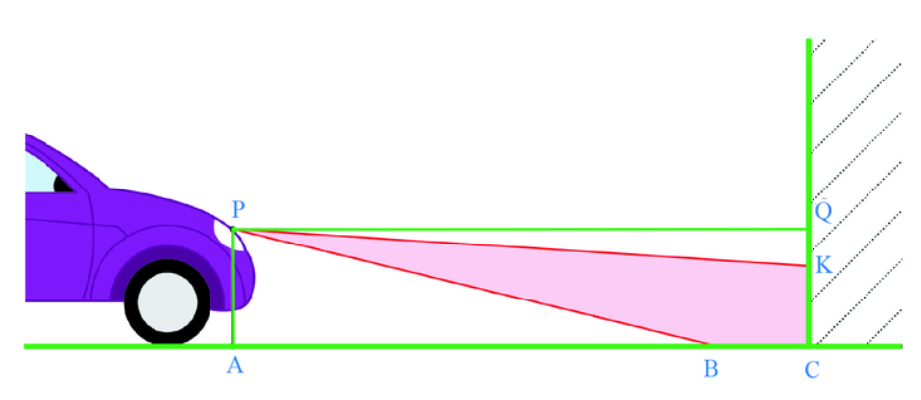
\includegraphics[scale=0.6]{trigo6.eps} 
\end{center}

Pauline réalise le schéma ci-dessous (qui n'est pas à l'échelle) et relève les mesures suivantes : \\
PA = 0,65 m, AC = QP = 5 m et CK = 0,58 m.\\
P désigne le phare, assimilé à un point.

\begin{center}
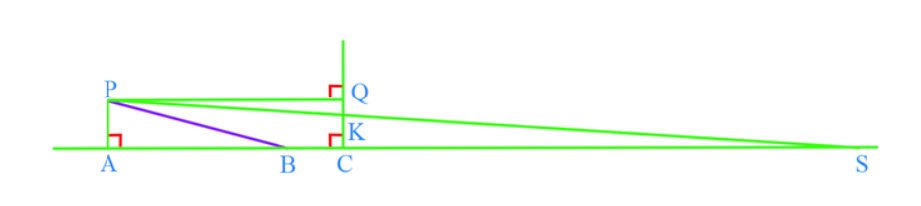
\includegraphics[scale=0.85]{trigo7.eps} 
\end{center}

Pour que l'éclairage d'une voiture soit conforme, les constructeurs déterminent l'inclinaison du faisceau. Cette inclinaison correspond au rapport $\frac{\mathrm{QK}}{\mathrm{QP}}$. Elle est correcte si ce rapport est compris entre 0,01 et 0,015.\\

\initq \q Vérifier que les feux de croisement de Pauline sont réglés avec une inclinaison égale à 0,014.\\

\q Donner une mesure de l'angle $\widehat{\mathrm{QPK}}$ correspondant à l'inclinaison. On arrondira au dixième de degré.\\

\q Quelle est la distance AS d'éclairage de ses feux ? Arrondir le résultat au mètre près.\\

\vspace*{0.5cm}

\end{document}
